\chapter{RELATED THEORY}

\section{Machine Unlearning}
Machine unlearning refers to a class of methods that remove the influence of specific training records from a trained model while preserving utility on non-removed data. The motivation is both regulatory and operational: privacy regulations such as the General Data Protection Regulation (GDPR) and the California Consumer Privacy Act (CCPA) establish the \textit{Right to be Forgotten}, giving users the legal right to request deletion of their personal data. Beyond compliance, practical machine learning pipelines frequently require removal of mislabeled, outdated, or sensitive samples after a model has already been deployed.

Formally, let $\mathcal{D} = \{z_1, z_2, \ldots, z_n\}$ denote a training dataset and let $\mathcal{A}(\mathcal{D})$ denote a learning algorithm that produces a model $\theta$. Given a subset $\mathcal{D}_f \subset \mathcal{D}$ of data points to be forgotten, the goal of machine unlearning is to produce a model $\theta'$ such that:

\[
\mathcal{A}(\mathcal{D} \setminus \mathcal{D}_f) \approx \mathcal{U}(\theta, \mathcal{D}_f, \mathcal{D})
\]

where $\mathcal{U}$ is the unlearning algorithm. In the exact unlearning setting, this approximation becomes an equality in distribution, meaning the unlearned model is statistically indistinguishable from a model retrained from scratch on $\mathcal{D} \setminus \mathcal{D}_f$.

In conventional machine learning, deletion is typically handled by retraining the model from scratch on the remaining dataset. While this approach is conceptually simple and guarantees complete removal of the target data's influence, it becomes impractical as models grow in size and datasets expand. Retraining a large model could take hours or days, making it impossible to honor deletion requests within reasonable timeframes, especially when multiple deletion requests arrive frequently.

Beyond computational efficiency, a practical unlearning system must address two additional concerns. First, \textit{verifiability} asks whether we can be confident that the target record no longer influences the model's predictions. Second, \textit{auditability} requires the system to maintain a clear, tamper-resistant record of deletion requests and their outcomes. In real-world deployments, this demands persistent bookkeeping structures that track active sample counts, shard assignments, and unlearning history, ensuring that model state remains consistent across repeated runs and system restarts.

\section{Taxonomy of Unlearning Approaches}

Machine unlearning methods can be broadly categorized into three families based on their underlying mechanism and the guarantees they provide.

\subsection{Exact Unlearning}
Exact unlearning methods guarantee that the resulting model is drawn from the same distribution as a model retrained from scratch on the remaining data. The SISA framework falls into this category. Exact unlearning is achievable when the training procedure can be decomposed into independent components, each of which can be retrained in isolation. The key condition is that the training data is partitioned such that each data point influences only one component of the final model.

\subsection{Approximate Unlearning}
Approximate unlearning methods aim to produce a model that is close to the exactly unlearned model, without the computational cost of full retraining. One prominent approach uses \textit{influence functions} to estimate the effect of removing a training point on model parameters. Given a model with parameters $\theta$ trained on dataset $\mathcal{D}$, the influence of removing a point $z$ on the parameters is approximated as:

\[
\Delta\theta \approx -\frac{1}{n} H_{\theta}^{-1} \nabla_\theta \ell(\theta, z)
\]

where $H_{\theta} = \frac{1}{n} \sum_{i=1}^{n} \nabla_\theta^2 \ell(\theta, z_i)$ is the Hessian of the training loss and $\ell(\theta, z)$ is the loss on point $z$. While theoretically elegant, computing the inverse Hessian is $\mathcal{O}(d^3)$ in the number of parameters $d$, making it computationally prohibitive for large models.

\subsection{Certified Data Removal}
Certified data removal, proposed by Guo et al., provides a formal privacy guarantee analogous to differential privacy. A mechanism $\mathcal{M}$ provides $(\epsilon, \delta)$-certified removal if for any dataset $\mathcal{D}$, any point $z \in \mathcal{D}$, and any set of outputs $\mathcal{S}$:

\[
\Pr[\mathcal{M}(\mathcal{D}) \in \mathcal{S}] \leq e^\epsilon \Pr[\mathcal{M}(\mathcal{D} \setminus \{z\}) \in \mathcal{S}] + \delta
\]

This guarantee ensures that an adversary cannot distinguish between a model trained on $\mathcal{D}$ and one from which $z$ has been removed, up to the privacy budget $(\epsilon, \delta)$. However, achieving tight certified removal bounds typically requires gradient-based updates and is most effective for convex models.

\section{SISA Framework for Efficient Unlearning}

The Sharded, Isolated, Sliced, and Aggregated (SISA) framework, introduced by Bourtoule et al., provides a structured approach to efficient machine unlearning by decomposing training into smaller, independently retrainable components. The core idea is straightforward: instead of training one monolithic model on the entire dataset, the dataset is divided into multiple independent \textit{shards}. Each shard is trained separately, producing its own sub-model. When a prediction is needed, the outputs from all shard models are aggregated, typically through majority voting for classification or averaging for regression.

\subsection{Sharding}
Given a dataset $\mathcal{D}$ of $n$ samples, the sharding step partitions $\mathcal{D}$ into $S$ disjoint subsets:

\[
\mathcal{D} = \mathcal{D}_1 \cup \mathcal{D}_2 \cup \cdots \cup \mathcal{D}_S, \quad \mathcal{D}_i \cap \mathcal{D}_j = \emptyset \; \forall \; i \neq j
\]

Each shard $\mathcal{D}_s$ contains approximately $\frac{n}{S}$ samples. The optimal number of shards $S$ can be estimated based on the dataset dimensionality $d$, total sample count $n$, and a configurable target samples-per-shard parameter $r$:

\[
S = \sqrt{\frac{d \cdot n}{r}}
\]

This formula balances the trade-off between retraining efficiency (favoring more shards) and model accuracy (favoring fewer, larger shards). A separate model $\theta_s$ is trained independently on each shard $\mathcal{D}_s$.

\subsection{Slicing}
To further reduce retraining time, each shard $\mathcal{D}_s$ is divided into $K$ time-ordered slices $\mathcal{D}_s^1, \mathcal{D}_s^2, \ldots, \mathcal{D}_s^K$. The model is trained incrementally, and the parameter state $\theta_s^k$ is saved after processing each slice $k$. When a deletion request targets a point in slice $k^*$, retraining begins from the saved state $\theta_s^{k^*-1}$ rather than from random initialization:

\[
\theta_s^{k^*}, \ldots, \theta_s^K \leftarrow \text{Retrain}(\theta_s^{k^*-1}, \mathcal{D}_s^{k^*} \setminus \{z\}, \mathcal{D}_s^{k^*+1}, \ldots, \mathcal{D}_s^K)
\]

This slicing mechanism provides an additional reduction in retraining time at the cost of increased storage for intermediate checkpoints.

\subsection{Aggregation}
At inference time, predictions from all $S$ shard models are combined. For classification tasks, majority voting is used:

\[
\hat{y} = \arg\max_c \sum_{s=1}^{S} \mathbf{1}[\hat{y}_s = c]
\]

For regression tasks, the final prediction is the average of shard predictions:

\[
\hat{y} = \frac{1}{S} \sum_{s=1}^{S} \hat{y}_s
\]

The key insight for unlearning is that any training record belongs to exactly one shard. Therefore, when a deletion request arrives, only the shard containing that record needs to be retrained, leaving all other shards untouched. This localized retraining dramatically reduces computational overhead compared to full model retraining.

\begin{figure}[H]
\centering
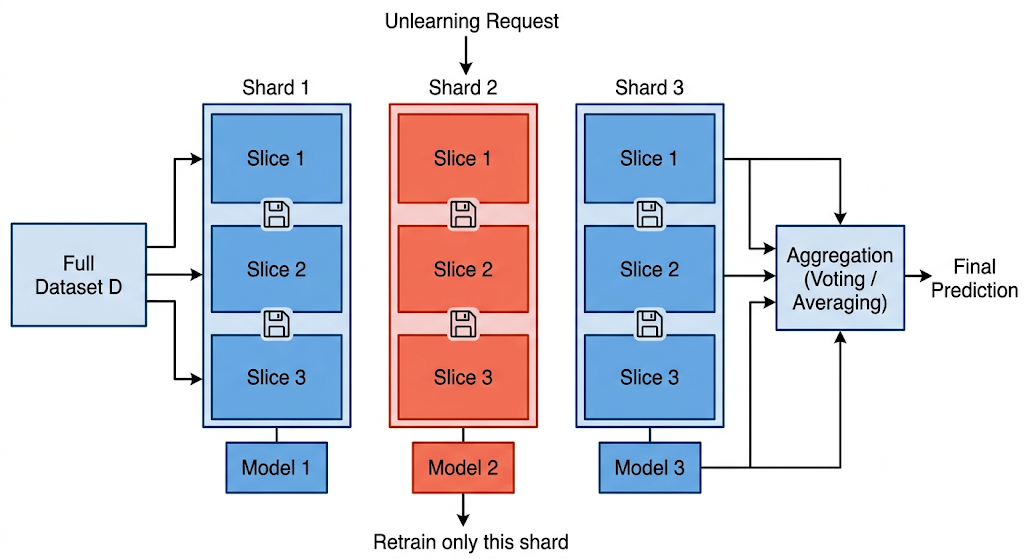
\includegraphics[width=0.95\textwidth]{Graphics/sisa_framework.png}
\caption{SISA Training Framework: Dataset partitioned into shards, each further divided into slices. On an unlearning request, only the affected shard is retrained from the last clean checkpoint.}
\label{fig:sisa_overview}
\end{figure}

\subsection{Unlearning Time Analysis}
Without SISA, the time to retrain a model after a single deletion request is $T$, the full training time. With SISA using $S$ shards and $K$ slices per shard, the expected retraining time for a uniformly random deletion request is:

\[
T_{\text{unlearn}} = \frac{T}{S} \cdot \frac{1}{K} \cdot \sum_{k=1}^{K} \frac{K - k + 1}{K} = \frac{T}{S} \cdot \frac{K+1}{2K}
\]

As $K \to \infty$, this approaches $\frac{T}{2S}$, meaning that with sufficient slicing, the expected retraining time approaches half the per-shard training time. This demonstrates that both sharding and slicing independently contribute to reducing unlearning overhead.

\section{Privacy Threat Models in Machine Learning}

Understanding why unlearning is necessary requires examining the privacy threats that trained models are susceptible to. Even after source data is deleted from storage, a deployed model may leak information about that data through several attack vectors.

\subsection{Membership Inference Attacks}
A membership inference attack attempts to determine whether a specific data point was part of the training set. Given a model $f_\theta$ and a target point $z$, an adversary constructs a binary classifier that predicts membership based on the model's output behavior, typically exploiting the observation that models tend to produce higher confidence predictions on training data than on unseen data. Formally, the adversary's advantage is:

\[
\text{Adv}_{\text{MI}} = \left| \Pr[\mathcal{A}(f_\theta, z) = 1 \mid z \in \mathcal{D}] - \Pr[\mathcal{A}(f_\theta, z) = 1 \mid z \notin \mathcal{D}] \right|
\]

A successful unlearning mechanism should reduce this advantage to near zero for any forgotten point $z \in \mathcal{D}_f$.

\subsection{Model Inversion Attacks}
Model inversion attacks attempt to reconstruct approximate representations of training data from model parameters or outputs. An adversary with access to a model $f_\theta$ can optimize an input $\hat{x}$ to maximize the predicted probability of a target class $c$:

\[
\hat{x} = \arg\max_x f_\theta(x)[c]
\]

This can reveal sensitive features of training samples, particularly in models trained on structured personal data. Unlearning a data point should ensure that such reconstruction no longer reflects the removed individual's information.

\section{Model Architectures Supporting Machine Unlearning}

The applicability of machine unlearning techniques varies across different model families, and the cost of unlearning depends heavily on how a model's training procedure can accommodate targeted retraining.

\subsection{Classical Machine Learning Models}
For classical machine learning on structured data, linear models and tree-based ensembles are particularly well-suited to SISA-style sharding. Linear models such as Logistic Regression and Ridge Regression have convex loss surfaces, meaning that retraining on a reduced shard converges reliably and predictably. The loss function for logistic regression on a shard $\mathcal{D}_s$ is:

\[
\mathcal{L}(\theta_s) = -\frac{1}{|\mathcal{D}_s|} \sum_{(x,y) \in \mathcal{D}_s} \left[ y \log \sigma(\theta_s^\top x) + (1-y) \log(1 - \sigma(\theta_s^\top x)) \right] + \frac{\lambda}{2} \|\theta_s\|^2
\]

where $\sigma(\cdot)$ is the sigmoid function and $\lambda$ is the regularization coefficient. Tree-based ensembles such as Random Forests and Gradient Boosting models are also well-suited, as each tree in the ensemble can be independently retrained on the affected shard without affecting other trees.

\subsection{Neural Network Architectures}
For neural network architectures, the landscape is more varied. Multi-Layer Perceptrons (MLPs) remain a common choice for tabular data and can be integrated into sharded training workflows with careful design. The forward pass of an MLP with $L$ layers is defined as:

\[
h^{(l)} = \sigma\left(W^{(l)} h^{(l-1)} + b^{(l)}\right), \quad l = 1, \ldots, L
\]

where $W^{(l)}$ and $b^{(l)}$ are the weight matrix and bias vector of layer $l$, and $\sigma$ is a non-linear activation function such as ReLU. Retraining an MLP shard requires backpropagation through all layers, which is more expensive than retraining a linear model but still significantly cheaper than retraining the full ensemble.

Convolutional neural networks (CNNs), such as the ResNet family, are prevalent in computer vision tasks but present additional challenges for unlearning. Their training involves complex optimization dynamics and dependencies across layers, making localized retraining less straightforward to implement without careful consideration of gradient propagation and initialization strategies.

\begin{figure}[H]
\centering
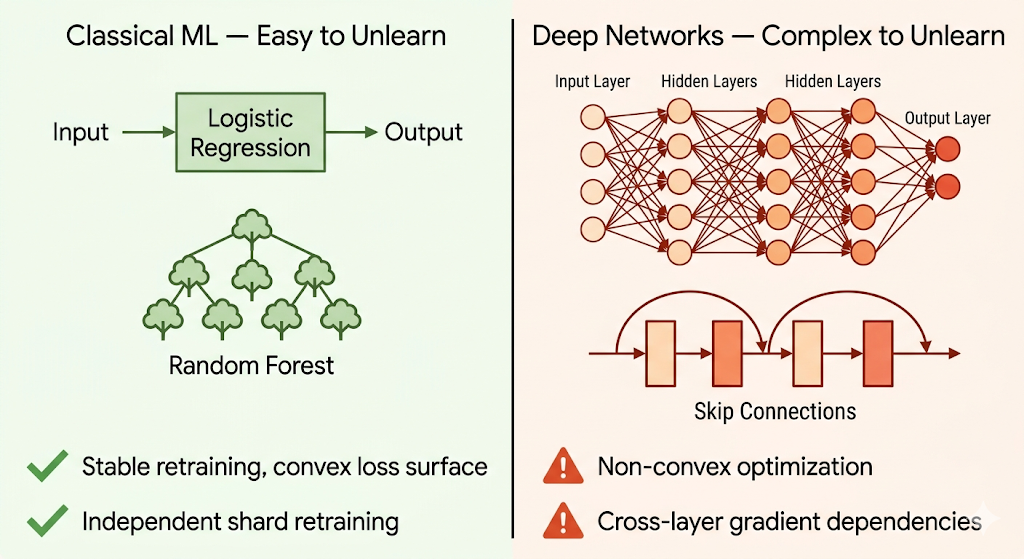
\includegraphics[width=0.95\textwidth]{Graphics/arch_comparison.png}
\caption{Comparison of model architectures and their suitability for SISA-based unlearning: classical models (left) offer stable retraining, while deep networks (right) introduce optimization complexity.}
\label{fig:arch_comparison}
\end{figure}

\subsection{Aggregation Strategies and Their Impact on Accuracy}
The choice of aggregation strategy affects both prediction accuracy and the robustness of the unlearning process. For classification, majority voting across $S$ shards produces a final prediction that is robust to individual shard errors, provided that the majority of shards produce correct predictions. The expected accuracy of the aggregated model under majority voting, assuming each shard achieves individual accuracy $p > 0.5$, is:

\[
P_{\text{agg}} = \sum_{k=\lceil S/2 \rceil}^{S} \binom{S}{k} p^k (1-p)^{S-k}
\]

This expression shows that aggregated accuracy increases with the number of shards $S$ when individual shard accuracy exceeds random chance, providing a theoretical justification for the SISA sharding strategy.

In practice, the choice between majority voting and weighted averaging depends on the nature of the task and the variance in shard model quality. When shards are of unequal size due to stratified sampling, assigning higher weights to larger shards can improve overall prediction quality. A weighted aggregation scheme assigns weight $w_s = \frac{|\mathcal{D}_s|}{n}$ to each shard model, yielding:

\[
\hat{y} = \sum_{s=1}^{S} w_s \cdot \hat{y}_s, \quad \sum_{s=1}^{S} w_s = 1
\]

This weighted scheme ensures that shards with more training data contribute proportionally more to the final prediction, reducing the impact of weaker models trained on smaller partitions.

Regardless of the specific architecture, the core requirement remains consistent: unlearning must enable removal of a record's influence by retraining only the minimally affected components rather than the entire model. The combination of sharding, slicing, and aggregation in the SISA framework provides a principled and practical solution that balances privacy guarantees, computational efficiency, and model accuracy. This project focuses primarily on scikit-learn compatible estimators for classical machine learning tasks, establishing a solid foundation that can be extended to neural architectures in future work. The theoretical principles discussed in this chapter directly inform the system design decisions, particularly around data partitioning, persistence, and audit logging.
